\part{Literature Review}
In this section, we provide a description of the key technologies used in this thesis. We begin by describing the Robot Operating System (ROS) and its functionality, followed by an overview of the navigation system employed, and a discussion of how the Open-RMF fleet management system operates.
\chapter{Overview of ROS1 and ROS2}
The Robotics Operating System (ROS)\footnote{\href{https://www.ros.org/}{https://www.ros.org/}} is an open-source collection of tools and libraries designed to support the development of robotics applications. Despite its name, ROS is not an operating system (OS) in the traditional sense, but rather a software development kit (SDK) that provides developers with a comprehensive set of tools for building robotic systems. It offers several features typically associated with an OS, including hardware abstraction, low-level device control, implementation of commonly used functionalities, inter-process communication, and package management.
The ROS ecosystem is built upon the following core components:
\begin{itemize}
	\item \textbf{Middleware communication layer (RMW)}: Built on the Data Distribution Service (DDS) standard, this layer enables nodes to exchange information using an anonymous publish/subscribe pattern. This design promotes fault isolation, separation of concerns, and modular interfaces. ROS also supports synchronous, Remote Procedure Call (RPC)-style communication between services.\\While the default DDS implementation is eProsima Fast DDS  (\texttt{rmw\_fastrtps\_cpp}), this work uses Eclipse Cyclone DDS (\texttt{rmw\_cyclonedds\_cpp}) due to its better compatibility with the Nav2 navigation stack in ROS Humble.
	\item \textbf{Development tools}: ROS provides a suite of tools for managing and enhancing software development, including utilities for launching, introspection, debugging, visualization, plotting, logging, and playback.
	\item \textbf{Multi-machine support} ROS includes tools and libraries for retrieving, building, writing, and executing code across multiple computers and OS.
	\item \textbf{Community and governance}: ROS is supported by an active and extensive global community, coordinated primarily by Open Robotics\footnote{\href{https://www.openrobotics.org/}{https://www.openrobotics.org/}}, which serves as the central organization for its development and maintenance.
\end{itemize}
\newpage
\section{Structure of ROS}
The official ROS documentation\footnote{\href{https://docs.ros.org/en/rolling/index.html}{https://docs.ros.org/en/rolling/index.html}} provides comprehensive information about the system.  All communication in ROS is handled through the \textbf{ROS Graph} , a peer-to-peer network of processes (called nodes) that execute concurrently and exchange information with one another. Some components of this graph are described below. Note that some of the functionalities described are specific to ROS 2 and are not available in ROS 1:
\begin{itemize}
	\item \textbf{Nodes}: A node is a modular process that performs a specific task. Nodes communicate with each other through topics, services, actions, and parameters. In ROS 2, nodes can be implemented as \textbf{LifecycleNode}\label{LifecycleNode}, which provide a managed state machine with defined transitions for startup and shutdown, enabling more deterministic behavior.
	\begin{figure}[h]
	\centering
	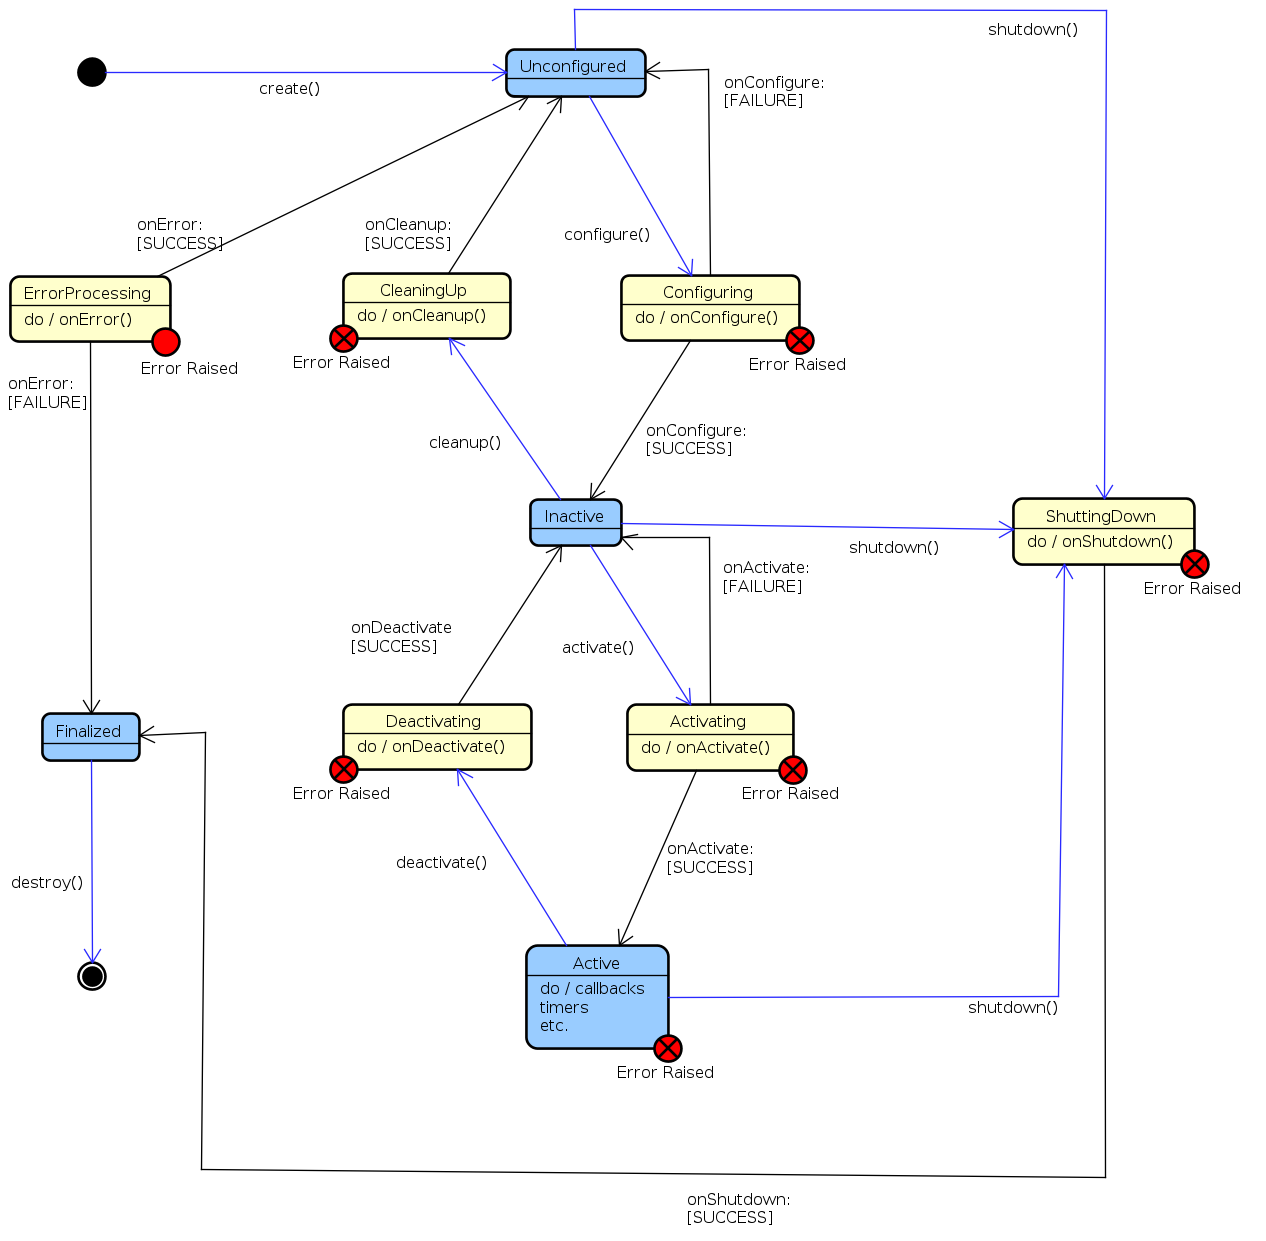
\includegraphics[width=1\linewidth]{img/life_cycle_sm_nf.png}
	\captionof{figure}{State Machine of LifecycleNode}
	\end{figure}\\
	Nodes can also be composed within the same process using the \textbf{Composition}\label{Composition} feature, which improves performance by bypassing middleware overhead\cite{macenski2023impactros2node}.
	\item \textbf{Topics}: Topics are used for communication between nodes to share streams of messages in a publisher-subscriber structure.
	\begin{center}
		\captionsetup{type=figure}
		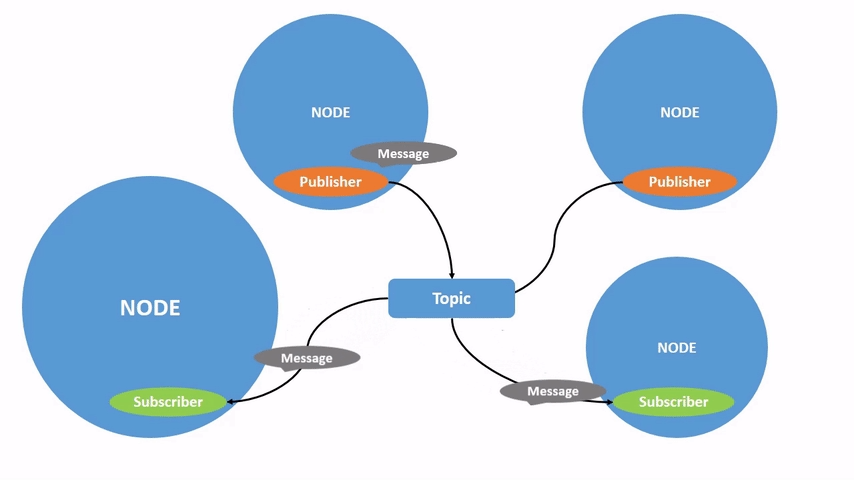
\includegraphics[width=0.6\linewidth]{img/Topic.png}
		\captionof{figure}{Topic process}
	\end{center}
	\item \textbf{Service}: Services are based on the request-response model. When a node with a service client sends a Request Message to a node with a service server, it receives a Response Message from that specific server.
	\begin{center}
		\captionsetup{type=figure}
		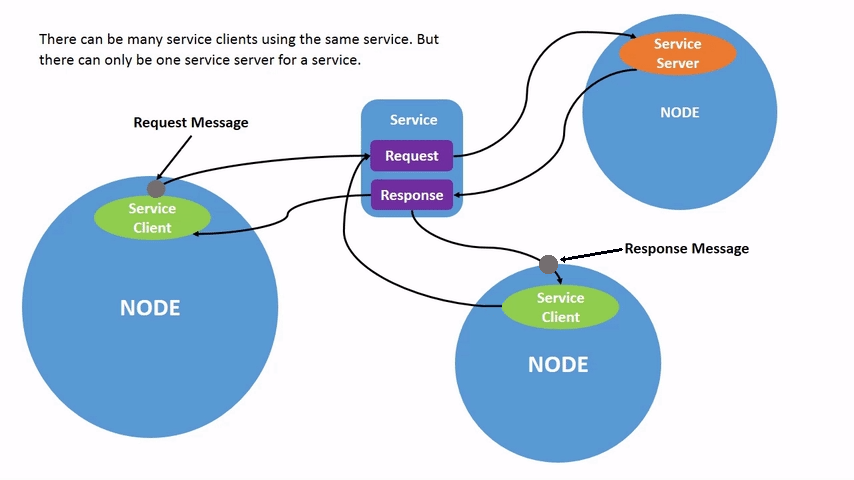
\includegraphics[width=0.6\linewidth]{img/Service.png}
		\captionof{figure}{Service process}
	\end{center}
	\item \textbf{Parameters}: Parameters are configurations of a node that can be modified without changing the source code.
	\item \textbf{Actions}\label{Action}: Actions are designed to support long-running tasks that require feedback and the capability to interrupt when needed. They combine two services (goal and result) and a publisher-subscriber mechanism (feedback). A node sends a goal request and receives an acknowledgment, then starts publishing feedback messages while executing the task, and finally the action server responds with the result.
	\begin{center}
		\captionsetup{type=figure}
		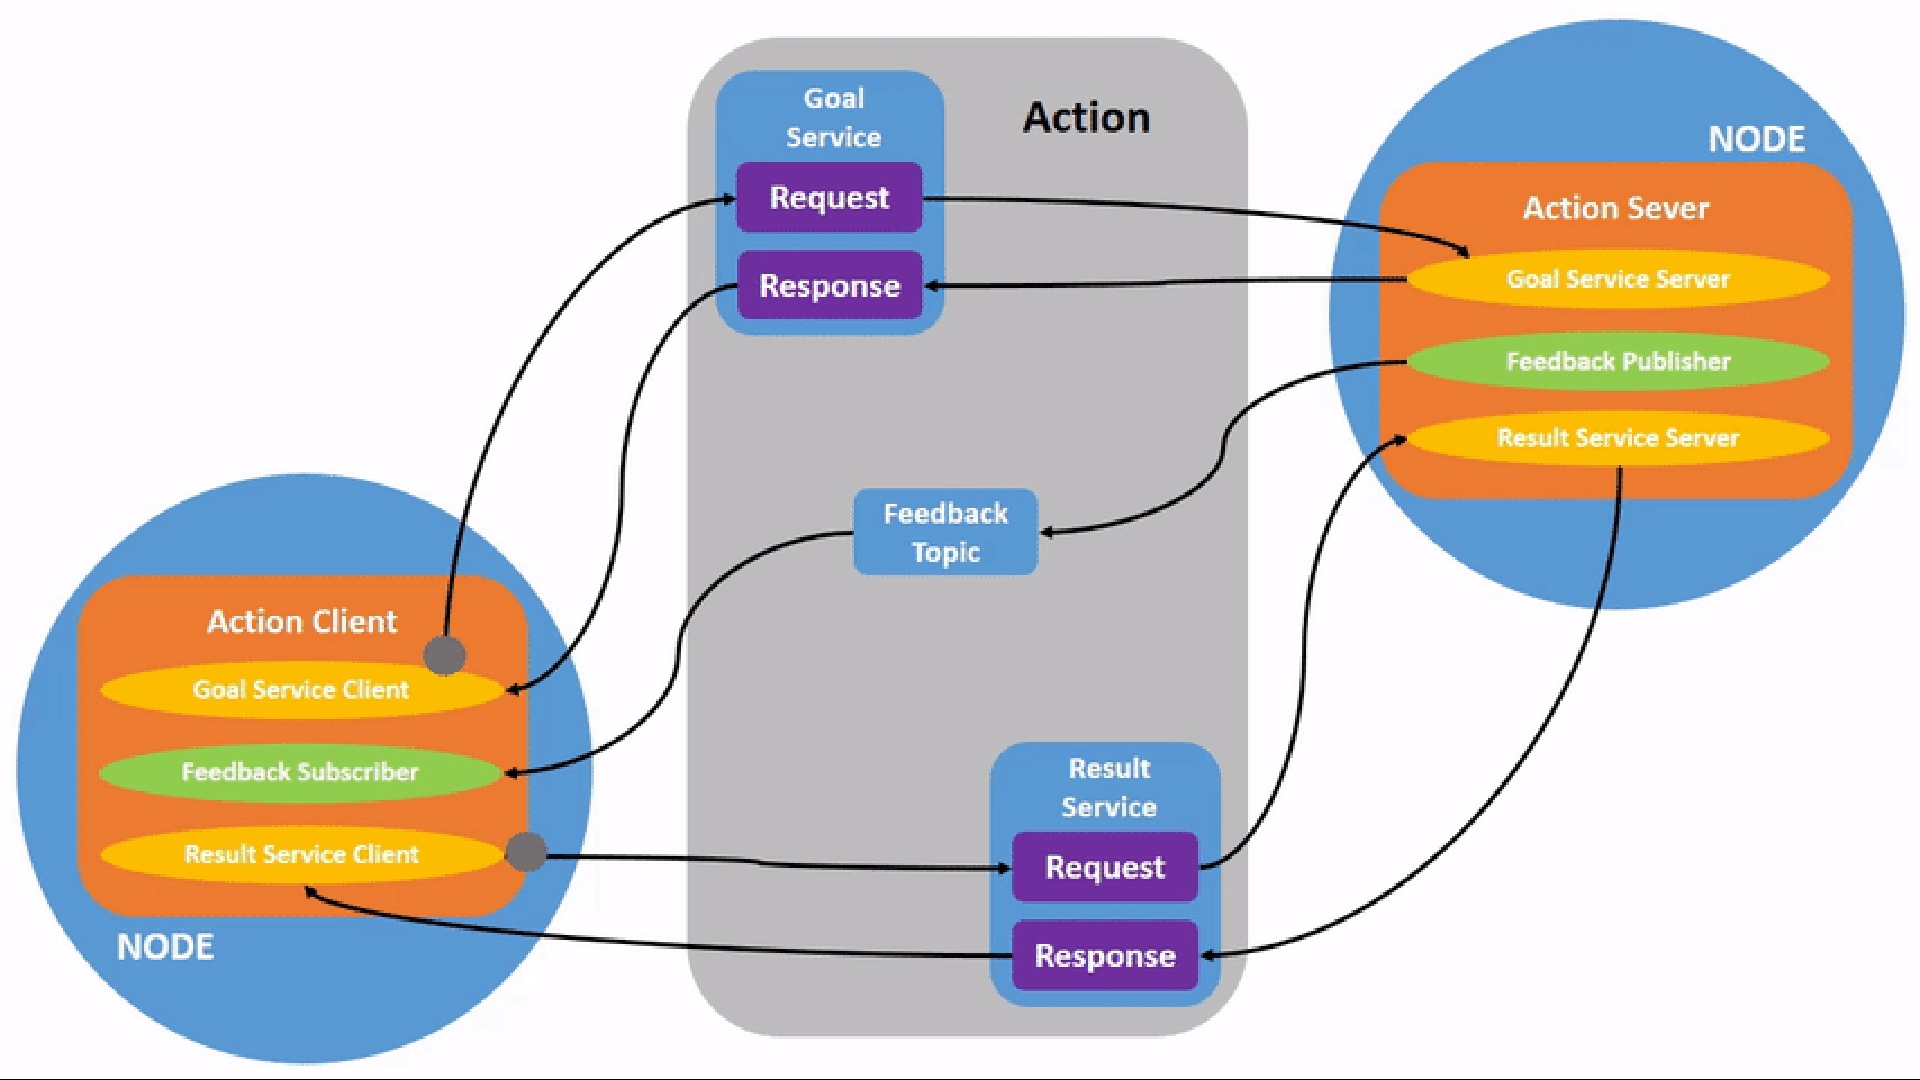
\includegraphics[width=0.6\linewidth]{img/Action.png}
		\captionof{figure}{Action process}
	\end{center}
\end{itemize}
\section{Tools of ROS}
This section describes the tools available in ROS for developing robotic systems:
\begin{itemize}
	\item \textbf{Launch}: A file structure that allows the simultaneous start of multiple nodes with a set of parameters.
	\item \textbf{rqt}: A graphical user interface (GUI) tool for ROS. It includes a series of plugins that facilitate development, monitoring, and diagnostics of the ROS system.
	\item \textbf{Rviz}: A 3D visualization tool for the Robot Operating System. It allows visualization of sensor data and state information from ROS.\\\\
	\begin{figure}[h]
		\centering
		\begin{subfigure}{0.4\textwidth}
		\centering
		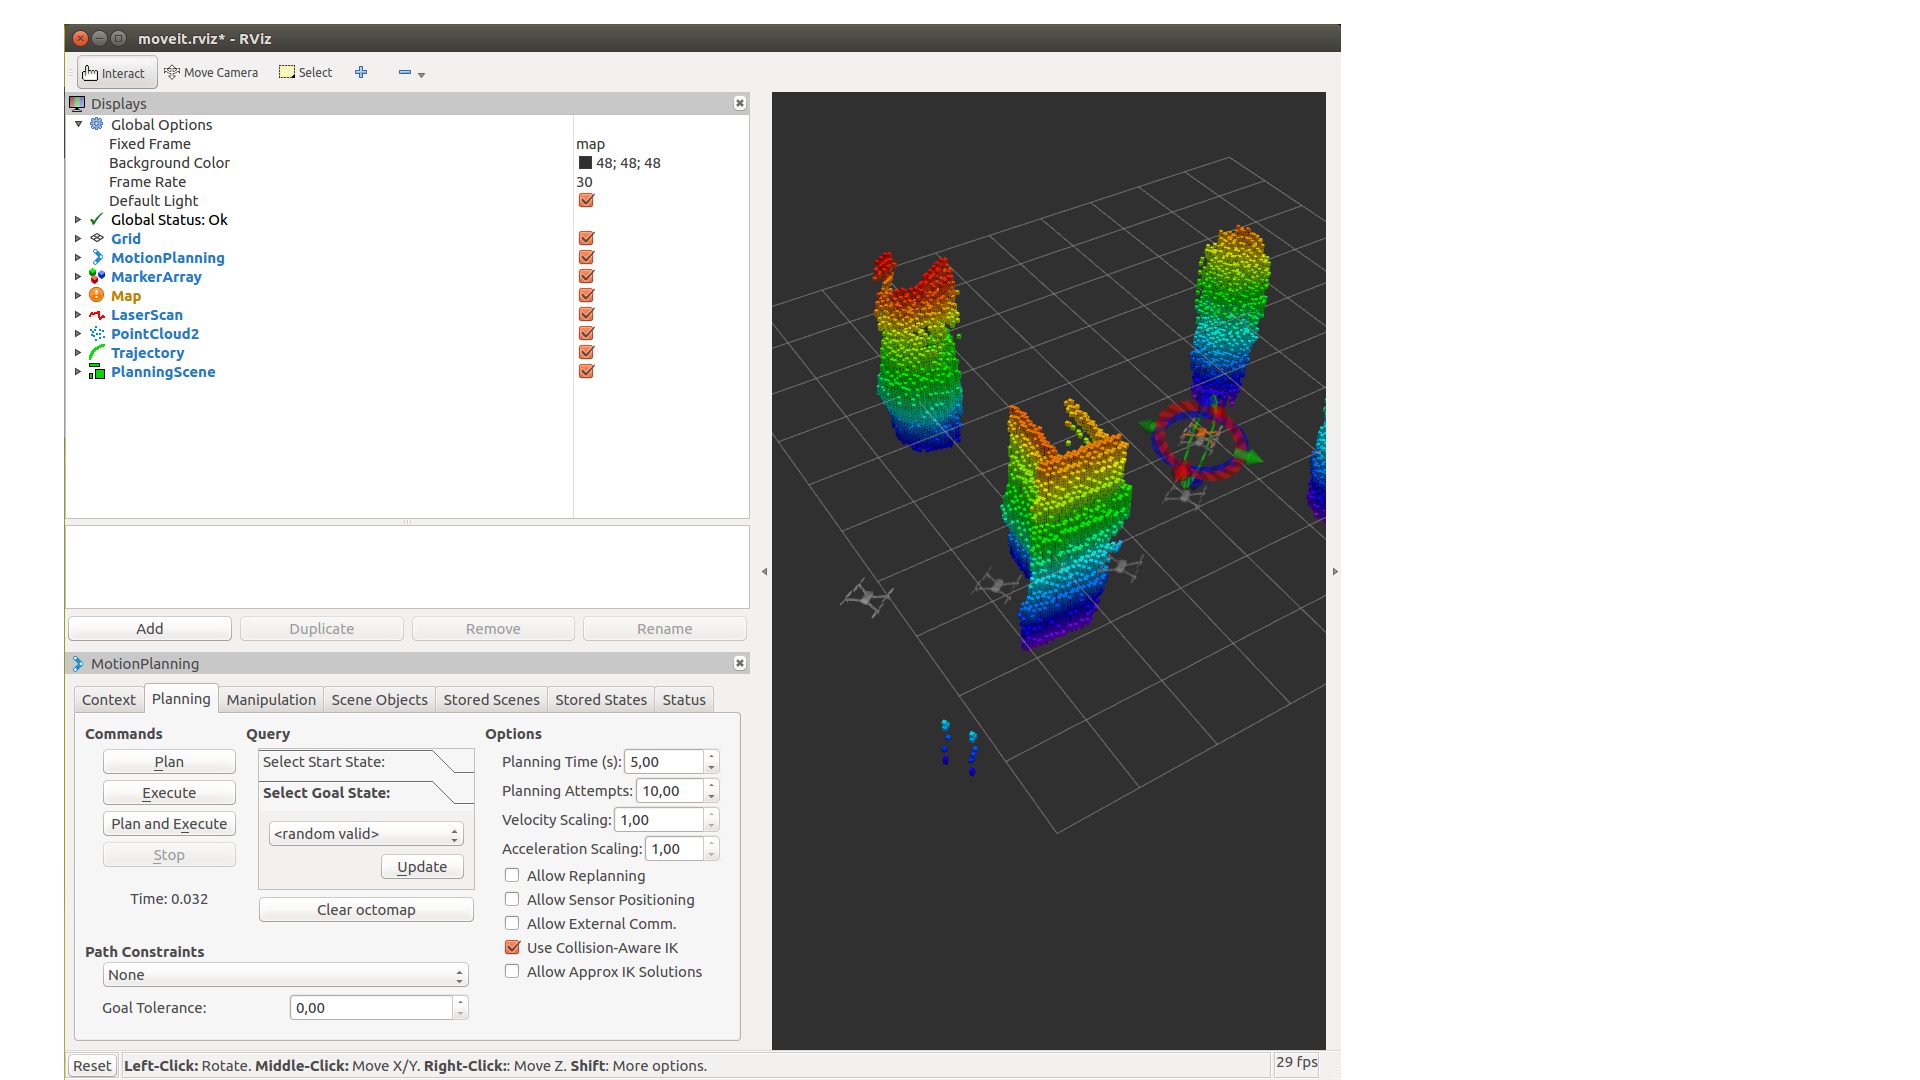
\includegraphics[width=1\linewidth]{img/rviz.png}
		\end{subfigure}
		\begin{subfigure}{0.4\textwidth}
		\centering
		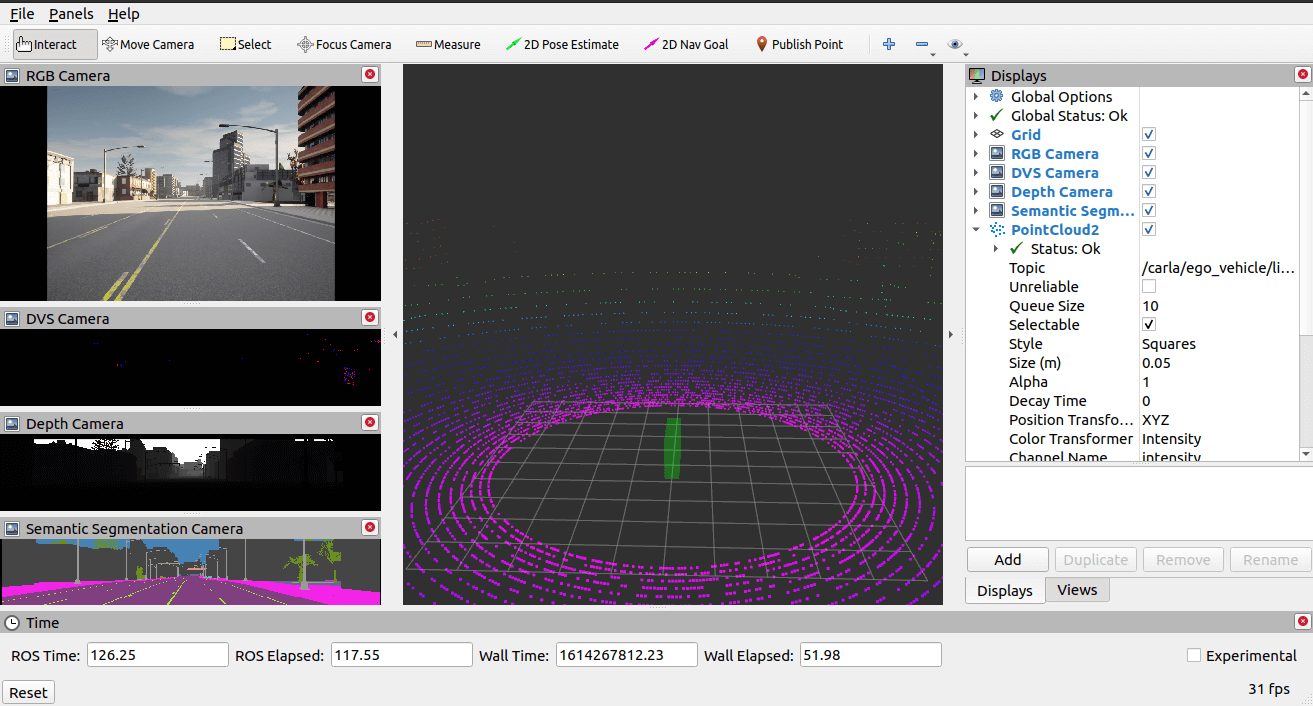
\includegraphics[width=1\linewidth]{img/rviz2.png}
		\end{subfigure}
		\captionof{figure}{Examples of visualization of ROS data with Rviz}
	\end{figure}\\
	\item \textbf{rosdep}: A command-line utility for installing system dependencies required by ROS packages.
	\item \textbf{sros2}: A security extension for ROS 2 that provides tools and instructions to apply security policies to DDS (Data Distribution Service).
\end{itemize}
Another important category of tools that are integrated with ROS is simulation environments. These environments allow developers to test their code on simulated robots under various conditions, which helps identify bugs that could potentially harm a real robot or its environment. Simulation tools provide realistic physical behavior for all components of a robotic system.
According to the ROS documentation, two main simulation tools are commonly used: Gazebo and Webots. Among them, Gazebo is also maintained by Open Robotics and is widely adopted in many projects, including the one discussed in this thesis.\\
Gazebo offer:
\begin{itemize}
	\item \textbf{ROS Integration}: A bridge that converts Protobuf messages to ROS messages, enabling communication between Gazebo and ROS.
	\item \textbf{Performance tools}: Features for distributed simulation across servers, dynamic asset loading, and adjustable time steps to optimize simulation performance.
	\item \textbf{Realistic simulation}: Support for a variety of sensors, including their noise models, within a 3D world rendered using OGRE 2.1\footnote{\href{https://wiki.ogre3d.org/Home}{https://wiki.ogre3d.org/Home}} and powered by multiple physics engine, the default one is DART\footnote{\href{https://dartsim.github.io/}{https://dartsim.github.io/}}.
	\item \textbf{Extensibility}: A modular design that supports plugins, allowing developers to run custom code that interacts directly with the simulation environment.	
\end{itemize}
	\begin{figure}[h]
		\centering
		\begin{subfigure}{0.4\textwidth}
			\centering
			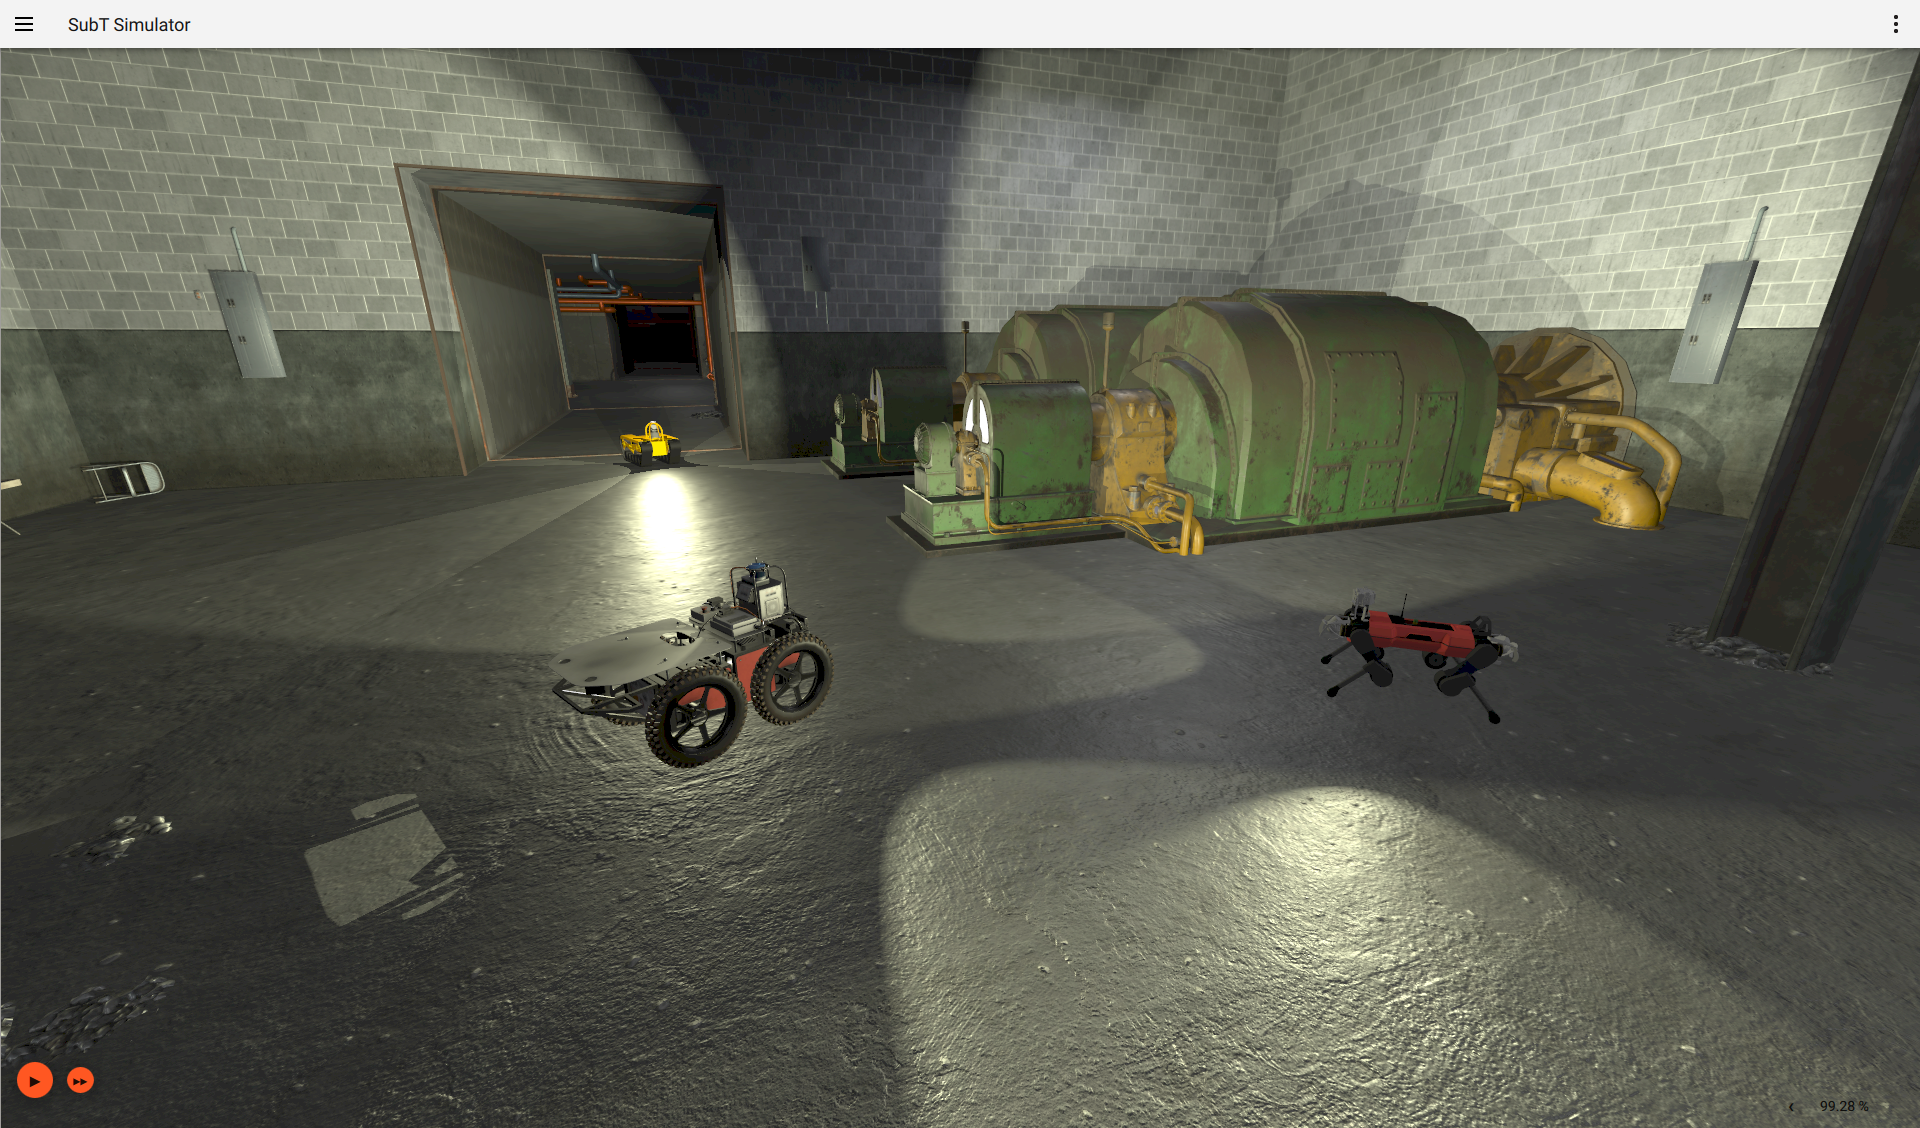
\includegraphics[width=1\linewidth]{img/gazebo1.png}
		\end{subfigure}
		\begin{subfigure}{0.4\textwidth}
			\centering
			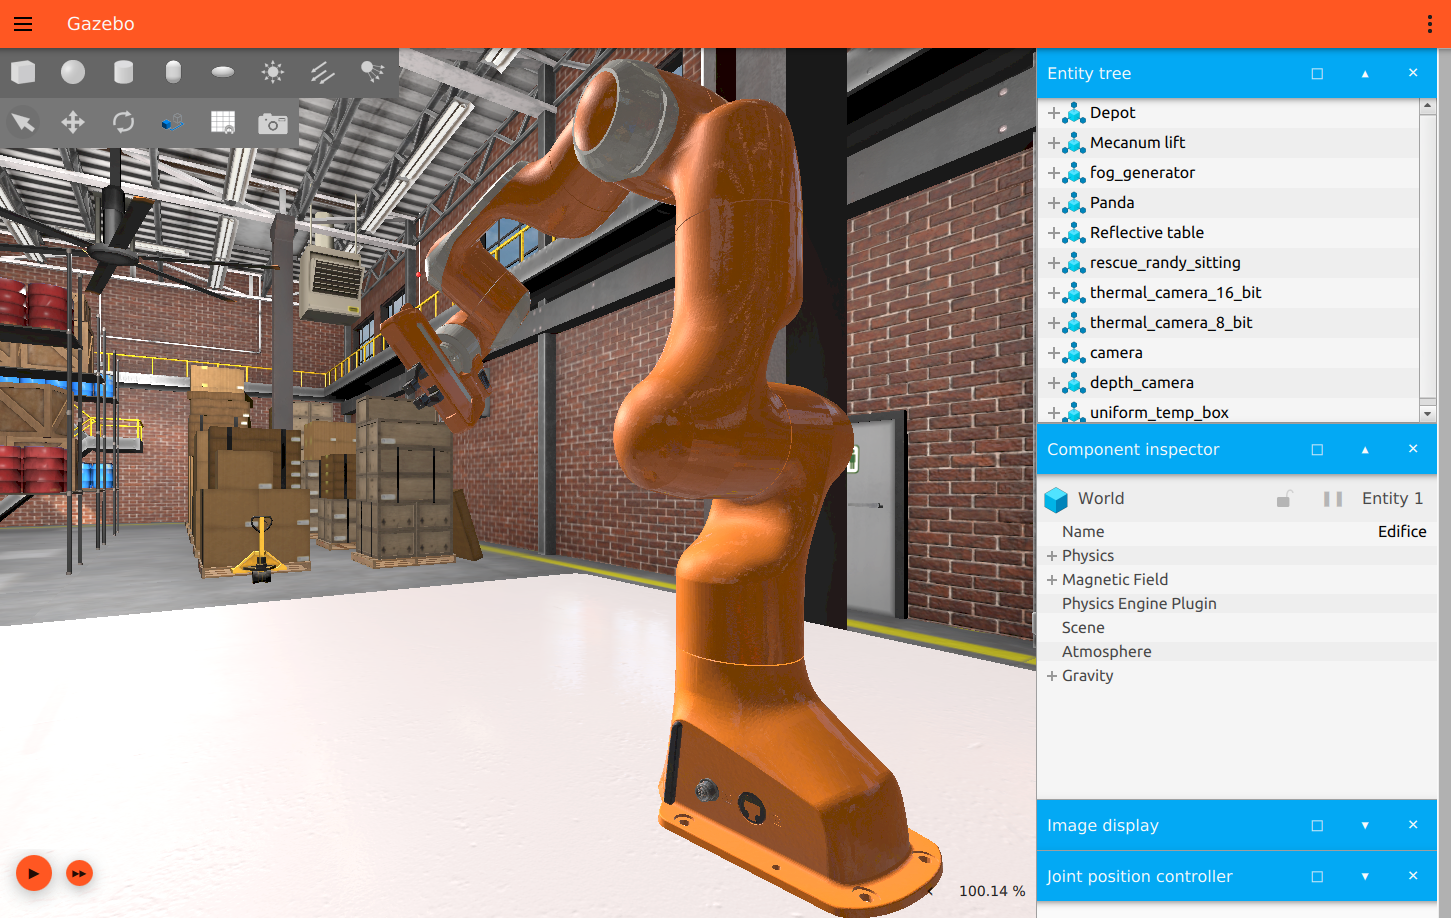
\includegraphics[width=1\linewidth]{img/gazebo2.png}
		\end{subfigure}
		\captionof{figure}{Examples of Gazebo}
\end{figure}
\chapter{Introduction to NAV2 and Google Cartographer}
Multiple tools are available to enable a robot to move autonomously within an environment. One of the most complete systems is Nav2 
\footnote{\href{https://nav2.org/}{https://nav2.org/}}
\cite{macenski2020marathon2}, the successor to the ROS 1 Navigation Stack.
\section{Description of Nav2}
Nav2 provides a comprehensive set of tools for perception, planning\cite{macenski2023survey}, control, localization, and visualization, allowing any robot to navigate autonomously and reliably, even in complex environments. It enables building a model of the environment from sensor data, dynamically calculating the optimal path to avoid obstacles, setting motor velocities, and executing navigation tasks using Behavior Trees.
\begin{figure}[h]
\centering
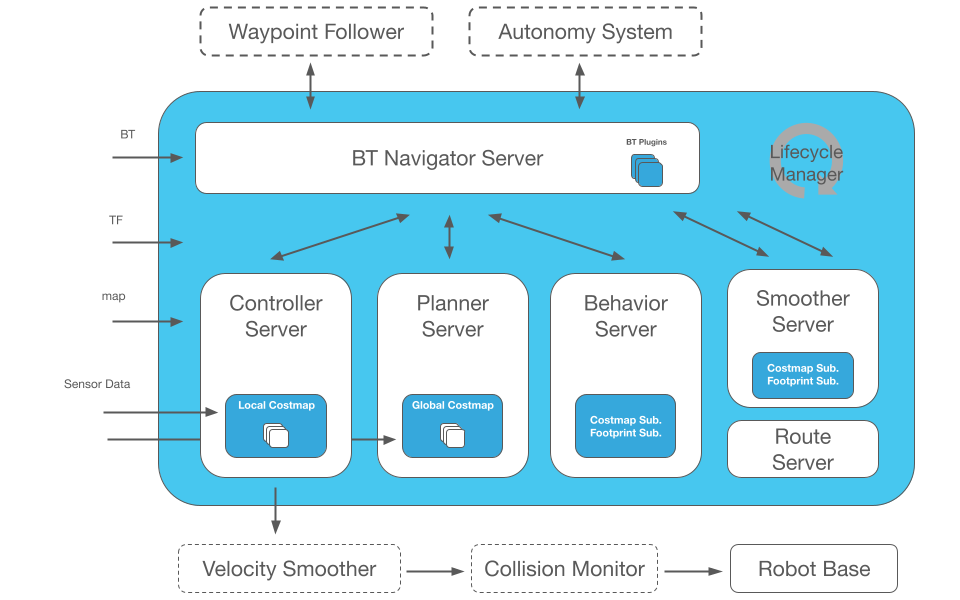
\includegraphics[width=0.8\linewidth]{img/nav2_architecture.png}
\captionof{figure}{Nav2 architecture} \label{Nav2Arch}
\end{figure}
\newpage
Nav2 introduces several improvements over ROS 1, including:
\begin{itemize}
	\item \textbf{Behavior trees}\cite{Colledanchise_2018}: Nav2 uses Behavior Trees to structure and execute tasks in a human-readable and modular way. These trees enable the creation of complex systems and can be tested with various tools. The  BehaviorTree.CPP\footnote{\href{https://www.behaviortree.dev/}{https://www.behaviortree.dev/}} library is used to implement them, and it allows linking different trees for flexible behavior management.
	\item \textbf{nav2\_util LifecycleNode}: This is a wrapper around the standard\\ \texttt{rclcpp\_lifecycle::LifecycleNode} described earlier \ref{LifecycleNode}. It adds a bond connection to the Lifecycle Manager, which monitors the state of each node and can safely transition nodes through their lifecycle states in the event of a failure.
	\item \textbf{Action Server}: Described in \ref{Action}, Nav2 uses action servers for Behavior Tree interactions, such as NavigationToPose (navigate to a specific location) and NavigationThroughPoses (navigate through multiple waypoints).
\end{itemize}
Nav2 is composed of several key nodes that work together to control the robot:
\begin{itemize}
	\item \textbf{Controller Server}: Handles movement requests. It uses plugin-based modules such as a progress checker (to verify if the robot is making progress), goal checker (to determine if the robot has reached its destination), and a controller (to generate velocity commands using the \textbf{local costmap} while avoiding collisions).
	\item \textbf{Planner Server}: Computes the global path to the destination using sensor data and a  plugin-based global planner loaded with the \textbf{global costmap}.
	\item \textbf{BT Navigator Server}: Implements the NavigateToPose, NavigateThroughPoses, and other task interfaces. It is a Behavior Tree-based implementation of navigation that is intended to allow for flexibility in the navigation task and provide a way to easily specify complex robot behaviors.
	\begin{figure}[h]
		\centering
		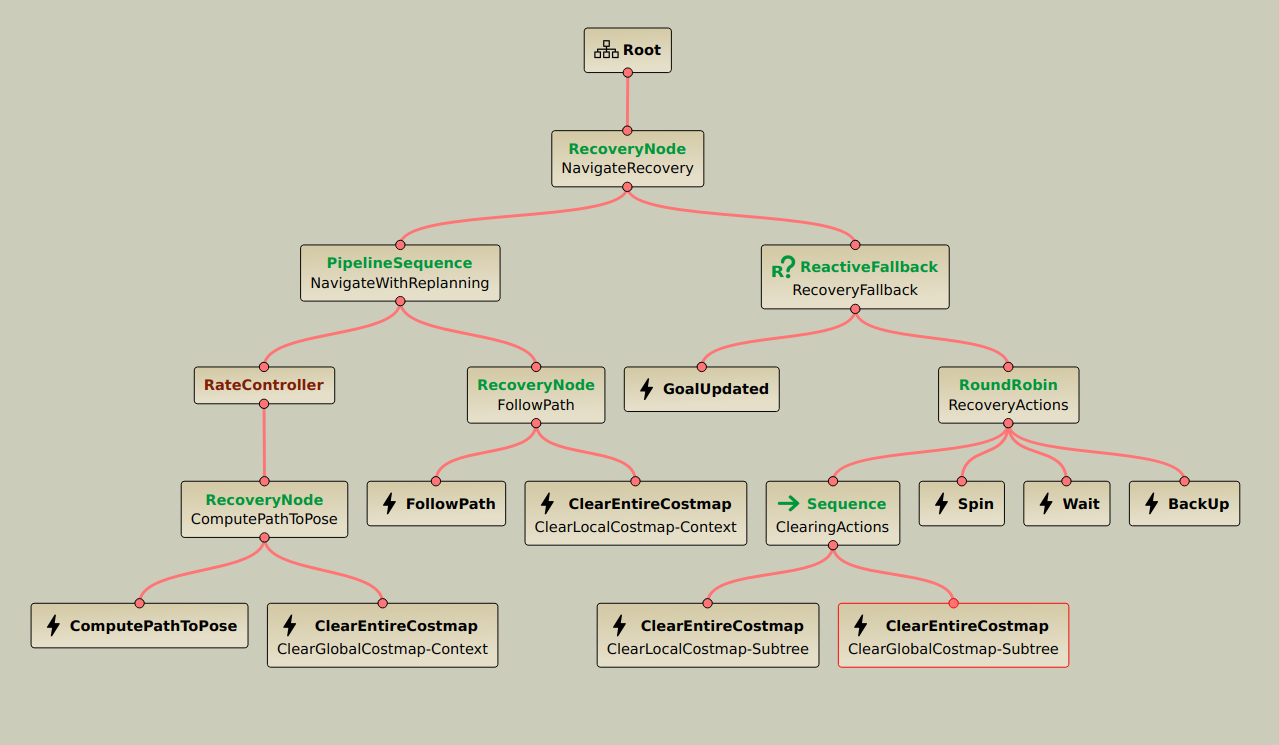
\includegraphics[width=0.72\linewidth]{img/bt_nav2_neg.humble.png}
		\captionof{figure}{Humble Nav2 BT navigation \texttt{navigate\_to\_pose\_w\_replanning\_and\_recovery.xml} loaded with Groot2}
	\end{figure}
	\item \textbf{Smoother Server}: Smooth the path minimizing sharp turns and rapid rotations.
	\item \textbf{Behavior Server}: Handles specific behavior actions like spinning, backing up, and waiting.
	\item \textbf{Waypoint Follower}: An example of orchestrated control (an \textbf{Autonomy System}), this node takes a list of waypoints and uses the NavigateToPose action server to move between them, optionally performing custom tasks (e.g., taking a photo) at each waypoint through plugins.
	\item \textbf{Route Server}: Calculates routes through a predefined navigation graph instead of using free-space planning.
	\item \textbf{Velocity Smoother}: Smooths velocity, acceleration, and deadband signals sent to the robot to ensure safe and smooth motion.
	\item \textbf{Costmap} is a representation of the environment using a regular 2D grid of cells with a cost (unknown, free, occupied, or inflated) and is used for generate the global plan or to compute local control efforts.
\end{itemize}
The next things that Nav2 relies on for controlling the navigation are:
\begin{itemize}
	\item \textbf{state estimation} of the robot that generate a suitable TF tree\label{TF_tree_nav2}, a tree structure of coordinate frames generated using the transform library\cite{6556373}, based on the \href{https://www.ros.org/reps/rep-0105.html}{REP 105}, that is should provide this structure: \texttt{map} $\rightarrow$ \texttt{odom} $\rightarrow$ \texttt{base\_link}. According to the REP 105 they are defines as:
	\begin{itemize}
		\item \texttt{map} : A world-fixed frame that may change in discrete jumps. It's useful for long-term global reference but not suitable for short-term localization.
		\item \texttt{odom} : A continuous world-fixed frame that may drift over time. It provides short-term local reference.
		\item \texttt{base\_link}: A robot fix frame.
	\end{itemize}
	The \texttt{odom} $\rightarrow$ \texttt{base\_link} link \label{ref_odom_to_base}can be estimated using various sensors. For improved accuracy, we use the \texttt{robot\_localization} package\cite{MooreStouchKeneralizedEkf2014}, which provides nonlinear state estimation using Kalman Filter fusing the robot's odometry and the IMU data.\\
	The \texttt{map} $\rightarrow$ \texttt{odom} link can be generate with a global positioning system like Simultaneous Localization And Mapping (SLAM) method\cite{sh-p1-prelude} or using the one provided by Nav2, Adaptive Monte-Carlo Localization (AMCL). \label{ref_map_to_odom}
	\item \textbf{map} can either be preloaded or built dynamically using a SLAM method. One SLAM method systems is Google Cartographer, which will be described in the next section. It is also the SLAM method that was used to generate the map for navigation.
\end{itemize}
\subsection{Cartographer}
Cartographer\cite{45466} is a SLAM method that operates using two main subsystems: a \textbf{Local SLAM} (called \textbf{Frontend}) that build a series of locally consistent \textbf{submaps} from successive scans and from the pose extrapolator with the possibility that it can drift during acquisition and a \textbf{Global SLAM} (called \textbf{Backend}) that reduces drift by performing loop closure—detecting when the robot has returned to a previously visited location. It uses scan matching against submaps and applies global optimization to align all submaps consistently and build a globally accurate map. Cartographer is capable of achieving mapping accuracy of 5 cm, but it requires extensive parameter tuning to reach optimal performance. 
\begin{figure}[h]
	\centering
	\includegraphics[width=1\linewidth]{img/Alg\_Cartographer.png}
	\captionof{figure}{Cartographer Algorithm}
\end{figure}
\chapter{Review of related work on porting navigation stack from ROS 1 to ROS 2}
The widespread adoption of the Robot Operating System (ROS) has introduced new use cases that were not originally considered during its development. Initially created as an academic project, ROS encountered limitations as users began applying it to more complex scenarios such as fleet management, deployment on embedded boards and microcontrollers, real-time systems, unreliable networks, and industrial applications. These emerging requirements highlighted architectural constraints in ROS 1, ultimately necessitating a complete redesign, which led to the development of ROS 2. Comprehensive documentation for ROS 2 is available at \href{https://design.ros2.org/}{https://design.ros2.org/} . Many companies have adopted the ROS 2 ecosystem, noting improvements in development workflows\cite{Macenski_2022} and in specific subsystems like in  Nav2\cite{macenski2023survey}. New initiatives, such as micro-ROS\footnote{\href{https://micro.ros.org/}{https://micro.ros.org/}}, aim to bring ROS 2 capabilities to microcontrollers. Additionally, features like Node Composition offer improved performance optimization\cite{macenski2023impactros2node} while sros2 allow for a better security\cite{vilches2022sros2usablecybersecurity}.
As outlined in these references, ROS 2 offers substantial advantages over ROS 1, making it the preferred framework for modern robotic applications. With this in mind, we will migrate the global planner using the official ROS 2 documentation\footnote{\href{https://docs.ros.org/en/rolling/How-To-Guides/Migrating-from-ROS1.html}{https://docs.ros.org/en/rolling/How-To-Guides/Migrating-from-ROS1.html}} and various secondary sources \footnote{\href{https://industrial-training-master.readthedocs.io/en/melodic/\_source/session7/ROS1-to-ROS2-porting.html}{https://industrial-training-master.readthedocs.io/en/melodic/\_source/session7/ROS1-to-ROS2-porting.html}}. 

\chapter{Overview of open source fleet management systems, particularly Open-RMF}
Currently, several fleet management systems are available:
\begin{itemize}
	\item \textbf{Isaac Mission Dispatch}\footnote{\href{https://github.com/NVIDIA-ISAAC/isaac_mission_dispatch}{https://github.com/NVIDIA-ISAAC/isaac\_mission\_dispatch}}: A microservice-enabled fleet management system developed by NVIDIA that allows users to submit missions to multiple robots and monitor both robot and mission statuses. It provides connectivity between robots and the fleet management system but does not handle logistics such as task allocation or conflict resolution (e.g., intersecting robot paths). The implementation relies on the VDA5050 protocol, an industry standard for communication between cloud control services and mobile robots, and uses MQTT, a lightweight, publish-subscribe network protocol designed for devices with limited resources and bandwidth.	
	\item \textbf{ROOSTER Fleet Management}\footnote{\href{https://github.com/ROOSTER-fleet-management}{https://github.com/ROOSTER-fleet-management}}:An open-source ROS 1-based project that supports heterogeneous fleet management with task allocation, scheduling, and routing functionalities.
	\item \textbf{Open Robotics Middleware Framework (Open-RMF)}\footnote{\href{https://www.open-rmf.org/}{https://www.open-rmf.org/}}: A free, open-source, and modular system that facilitates interoperability between multiple robot fleets and physical infrastructure such as doors, elevators, and building management systems.
	\item \textbf{Robofleet}\footnote{\href{https://github.com/ut-amrl/robofleet}{https://github.com/ut-amrl/robofleet}}\cite{sikand2021robofleetopensourcecommunication}: An open-source system based on ROS 1 that supports inter-robot communication, remote monitoring, and remote tasking for heterogeneous fleets of ROS-enabled service robots. It is specifically designed to handle network variability and to incorporate security control features.
	\item \alert{\textbf{openTCS}\footnote{\href{https://opentcs.org}{https://opentcs.org}}: open Transportation Control System) is a free control system software for coordinating fleets of automated guided vehicles (AGVs) and mobile robots. It can control any automatic vehicle,independent of their specific characteristics, with communication capabilities. Also, It can manage vehicles of different types and performing different tasks at the same time.}
\end{itemize}
Other frameworks provide the infrastructure needed to initiate fleet control:
\begin{itemize}
	\item \textbf{Transitive Robotics}\footnote{\href{https://transitiverobotics.com/}{https://transitiverobotics.com/}}: An open-source framework for full-stack robotics, designed to simplify the development of capabilities that connect robots, cloud services, and web front-ends through a dynamically updating shared data model. It addresses common challenges in building full-stack robotic applications, such as unreliable networks, intermittently offline robots, and cross-device versioning.
	\item \textbf{Robot Web Tools}\footnote{\href{https://robotwebtools.github.io/}{https://robotwebtools.github.io/}}: A collection of tools that enable communication with remote robots via web technologies, facilitating remote monitoring and interaction.
\end{itemize}
Given that Open-RMF offers control over multiple fleets, enables structured interaction between them to achieve optimal outcomes, provides a comprehensive toolset for system development, is based on ROS 2, and is open source, it will be used as the foundation for our fleet management architecture.
\section{Open-RMF description}
Open-RMF is a flexible and modular toolkit built on ROS 2 that facilitates interaction between heterogeneous robot fleets. It employs standardized protocols to enable communication with infrastructure, environments, and automation systems, optimizing the utilization of critical shared resources such as elevators, doors, narrow corridors, and other robots. By coordinating access to these resources, Open-RMF introduces system-level intelligence that helps prevent conflicts and ensures proper task and resource allocation.
Figure \ref{fig:Open-RMF Structure} illustrates the architecture and operational workflow of Open-RMF.
\begin{figure}[h]
	\centering
	\includegraphics[width=0.8\linewidth]{img/RMF\_struct.png}
	\captionof{figure}{Open-RMF Structure}
	\label{fig:Open-RMF Structure}
\end{figure}
\\
The fleets that can be controlled through Open-RMF can be categorized into three types:
\begin{itemize}
	\item \textit{Full Control}: Fleets of this type provide full status updates and allow complete control over path planning and execution.
	\item \textit{Traffic Light}: These fleets also provide full status updates, but only allow limited control, such as pausing and resuming operations. Open-RMF has control over certain behaviors, but not over the specific paths.
	\item \textit{Read Only}: These fleets only provide status updates and cannot be controlled. Only one read-only fleet can exist in the system at any given time, as the presence of multiple read-only fleets would make it nearly impossible to avoid deadlocks or resource conflicts.
\end{itemize}
If a fleet lacks has \textit{No Interface}, it can lead to deadlocks in resource allocation and is incompatible with an RMF system.
\\
The core of Open-RMF, known as \texttt{rmf\_core}, is composed of several modular packages, each serving a distinct role within the system:
\begin{itemize}
	\item \texttt{rmf\_traffic}: Provides core scheduling and traffic management capabilities. It is based on a platform-agnostic \textbf{Traffic Schedule Database} and includes two main mechanisms for traffic deconfliction:
	\begin{figure}[h]
		\centering
		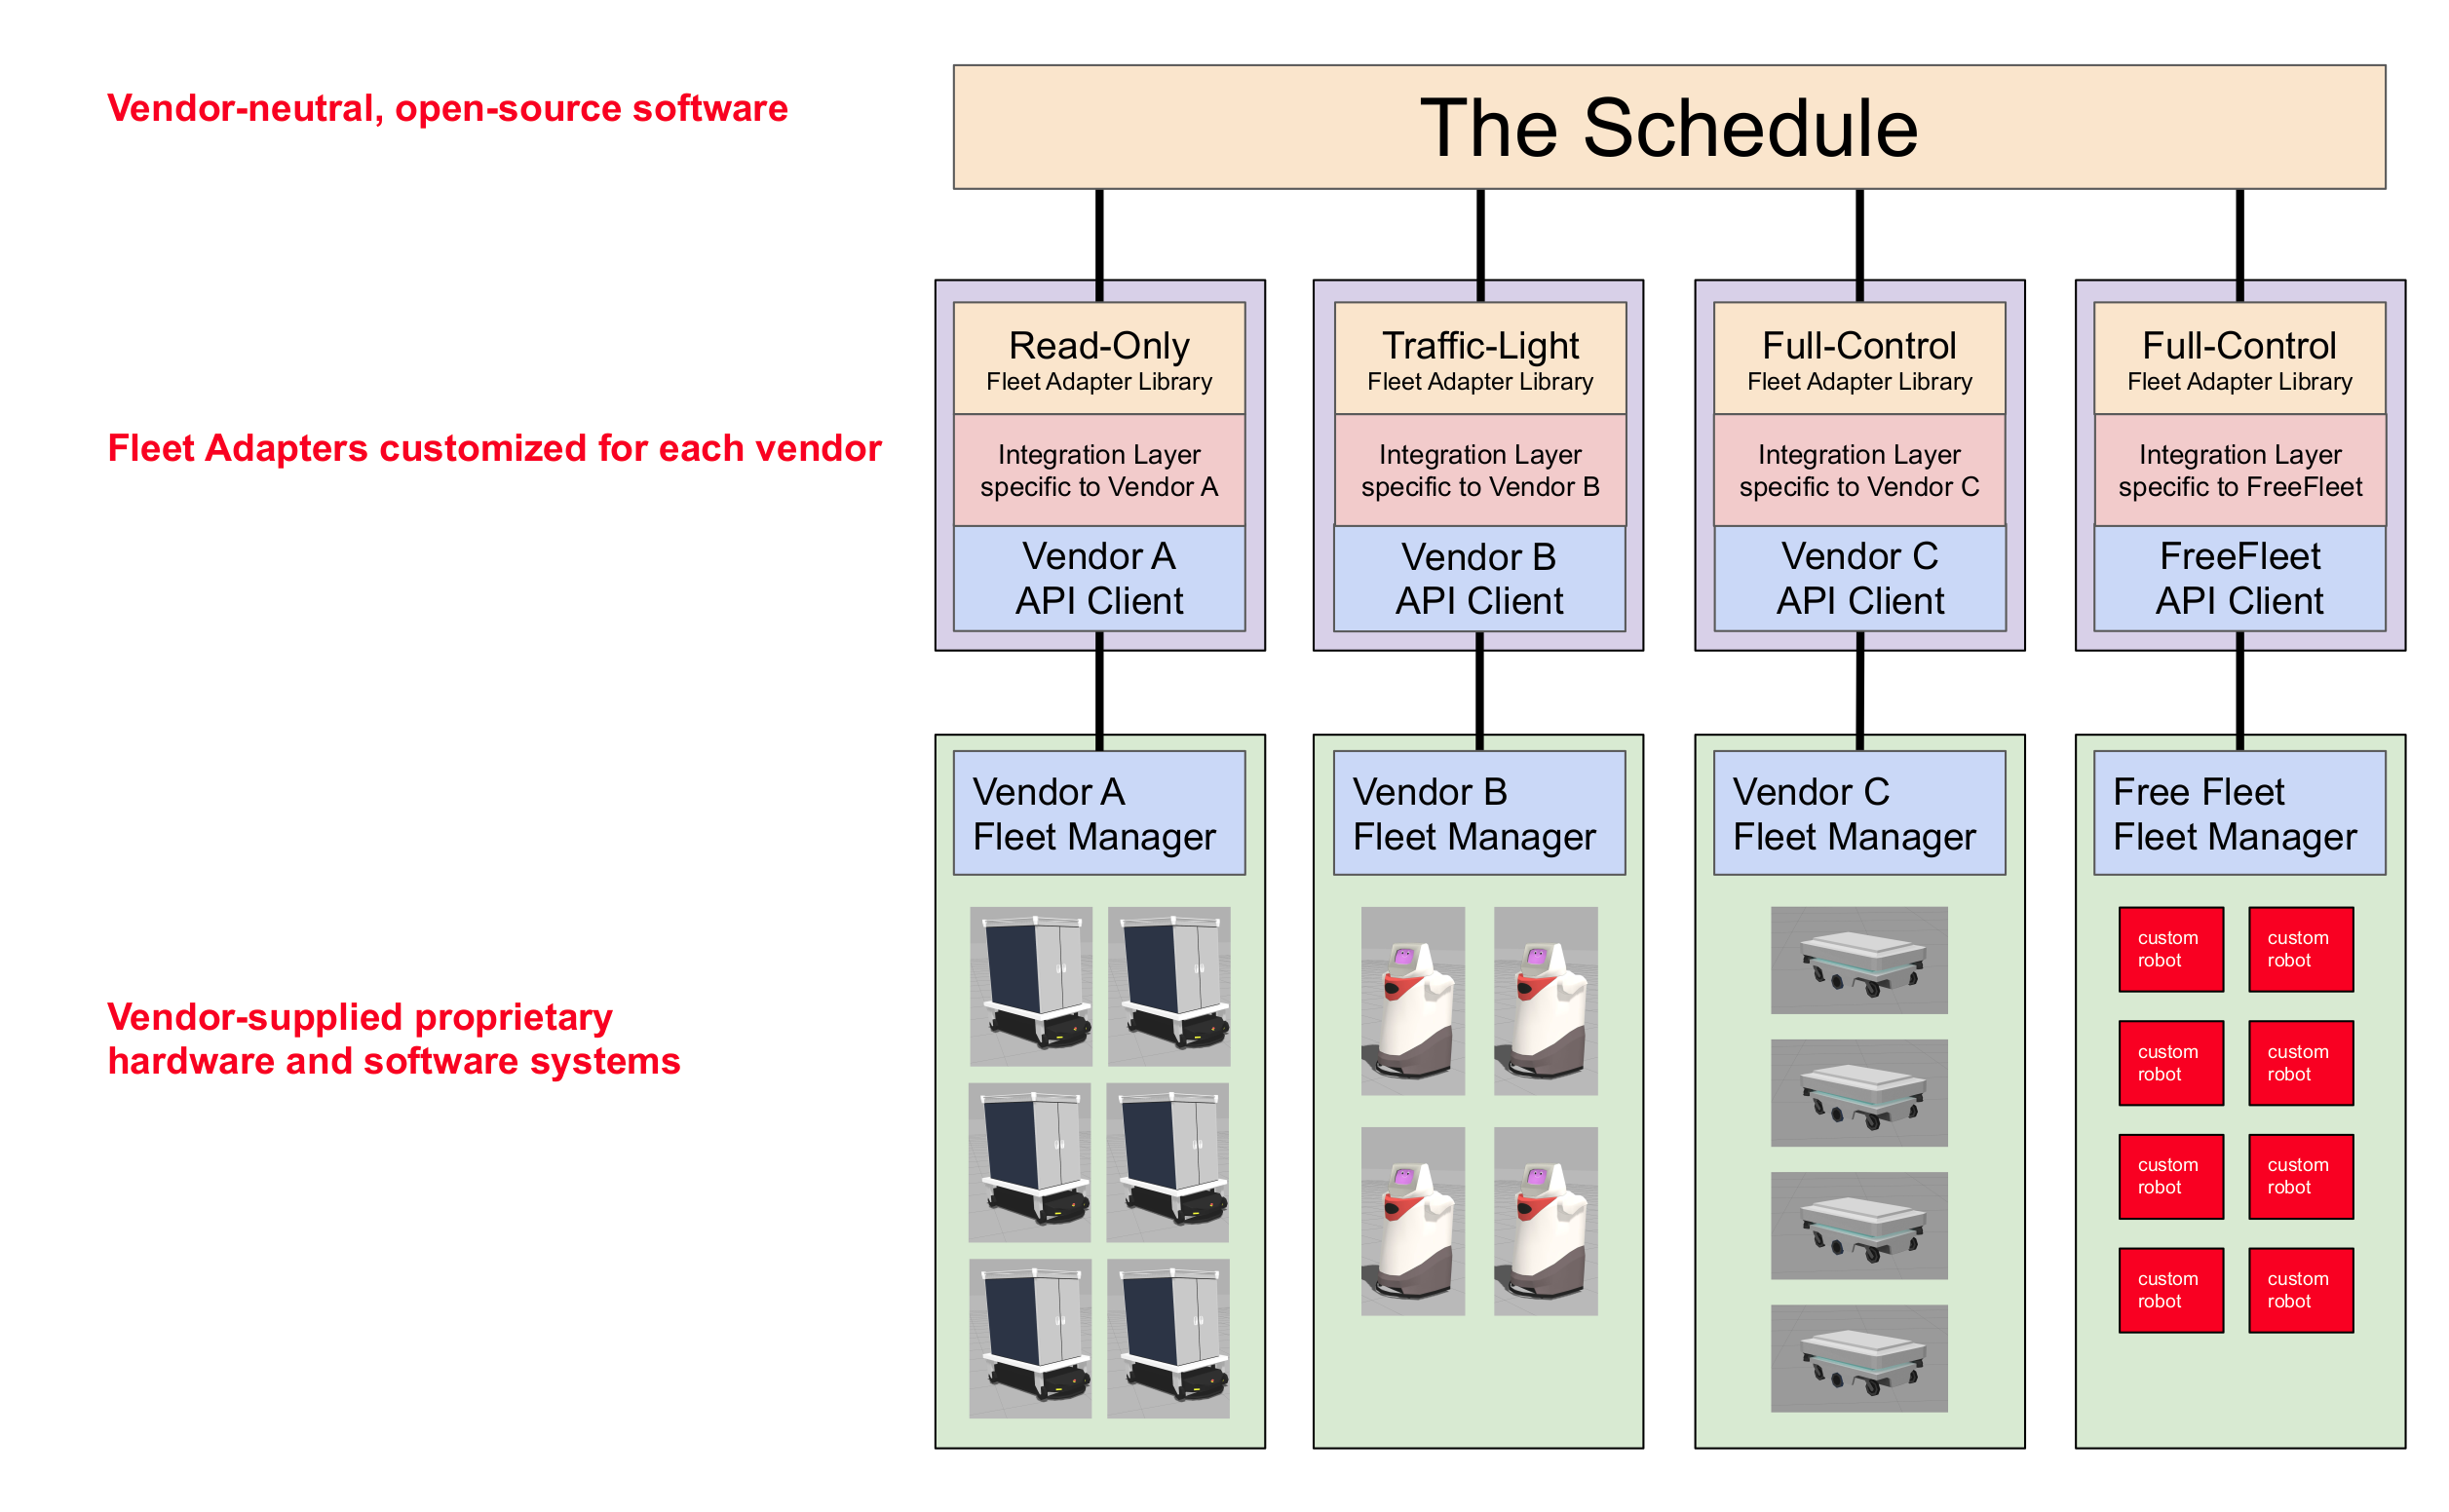
\includegraphics[width=0.8\linewidth]{img/RMF_tut_schedule.png}
		\captionof{figure}{Open-RMF Schedule structure}
		\label{fig:Open-RMF Schedule structure}
	\end{figure}
		\begin{itemize}
			\item \textit{Prevention}: When changes occur in the database (e.g., route cancellations), fleet managers can proactively replan routes to avoid conflicts.
			\item \textit{Negotiation}: When a potential conflict is detected between two or more schedule participants, a conflict notice is issued to the relevant fleet managers. Each manager responds with a preferred path that accommodates other agents, and an external arbitration module selects the optimal path.
		\end{itemize}
	Conflict avoidance for Automated Guided Vehicles (AGVs) is implemented using a time-dependent extension to A* search. This algorithm considers both spatial and temporal dimensions, allowing it to generate conflict-free paths by accounting for the future movements of other agents. Support for Autonomous Mobile Robots (AMRs) is under active development.
	\item \texttt{rmf\_traffic\_ros2}: Provides the necessary ROS 2 interfaces for integrating rmf\_traffic into ROS 2-based systems.
	\item \texttt{rmf\_task}: Contains APIs and base classes for defining and managing tasks in RMF.
	The framework natively supports three types of task requests:
	\begin{itemize}
		\item \textit{Clean}: For robots capable of cleaning floor spaces.
		\item \textit{Delivery}: For robots tasked with transporting items between locations.
		\item \textit{Loop}: For robots required to repeatedly navigate between two or more points.
	\end{itemize}
	\item \texttt{rmf\_dispatcher\_node}: Contains the logic responsible for task allocation and management across multi-fleet systems. When a user submits a new task request, the dispatcher intelligently assigns it to the most suitable robot by querying each fleet adapter capable of performing the task. These adapters respond with bids indicating which robot is best suited, and RMF uses this bidding mechanism to determine the optimal assignment, as illustrated in Figure \ref{fig:Open-RMF Bid Task}.
	\begin{figure}[h]
		\centering
		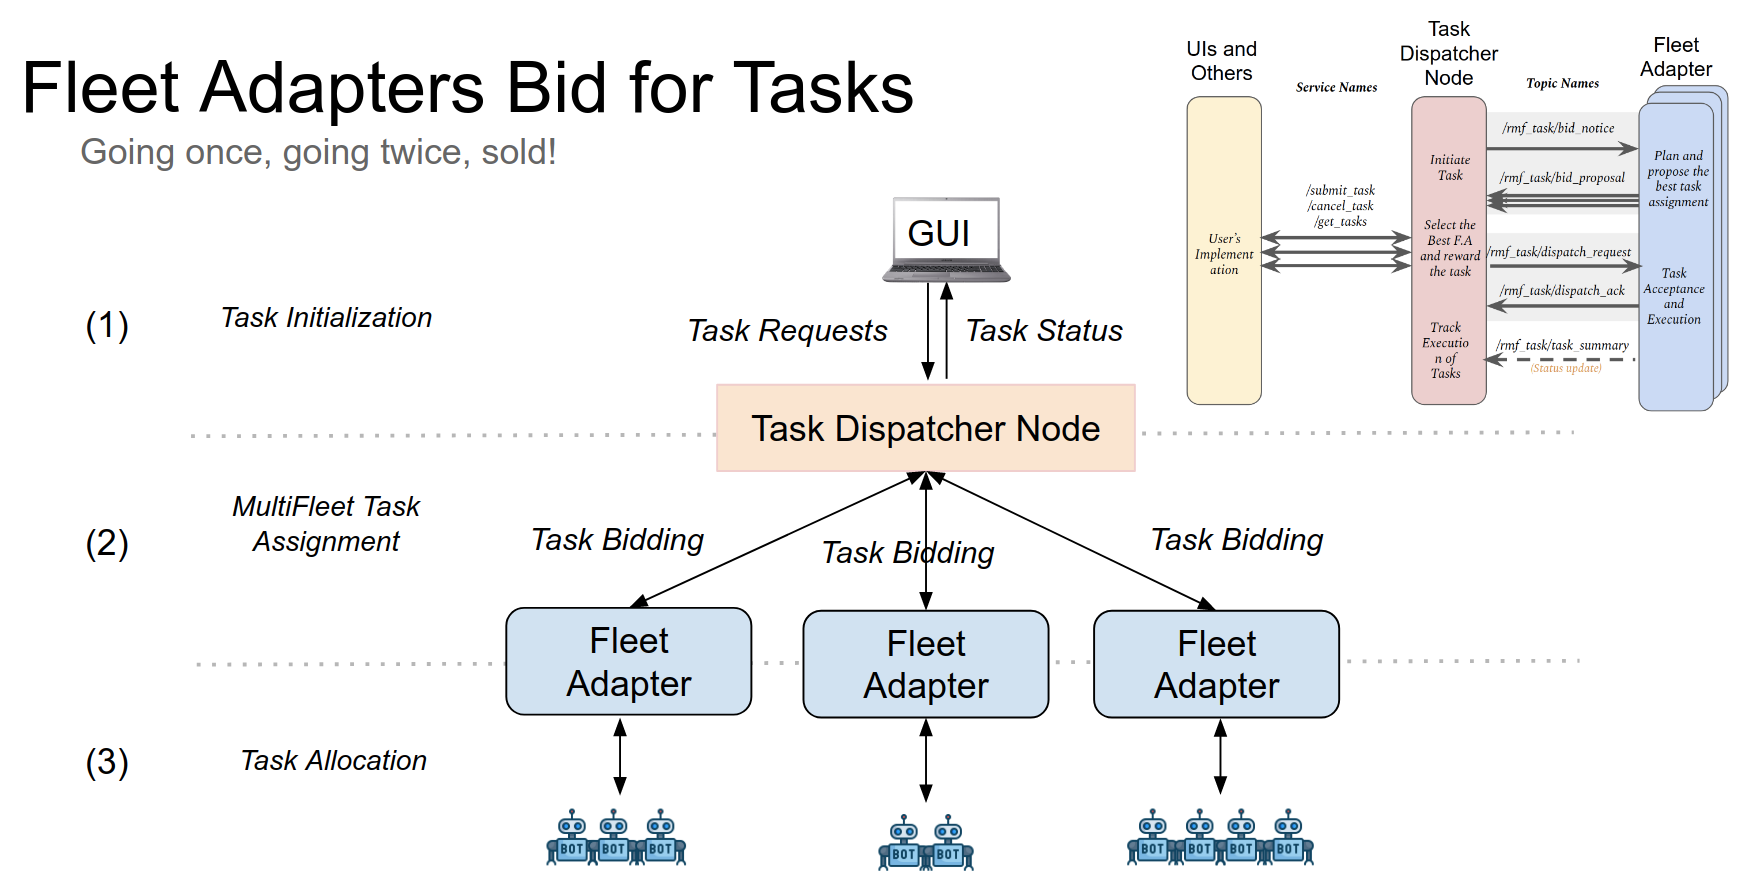
\includegraphics[width=0.8\linewidth]{img/RMF_tut_BidTask.png}
		\captionof{figure}{Open-RMF Bid Task}
		\label{fig:Open-RMF Bid Task}
	\end{figure}
	\item \texttt{rmf\_battery}: Provides battery consumption estimation models for different robot activities, aiding in energy-aware task planning.
	\item \texttt{rmf\_ros2}: Supplies ROS 2 adapters, nodes, and Python bindings to integrate the RMF core components into ROS 2 applications.
	\item \texttt{rmf\_utils}: A collection of utility functions and tools used across various RMF packages.
	
\end{itemize}

The following tools are available to support development with Open-RMF:
\begin{itemize}
	\item \textbf{RMF demos}: A collection of demonstration packages showcasing the capabilities of Open-RMF. These serve as a useful starting point for development and experimentation.
	\item \textbf{Traffic Editor}: A graphical map editor used to define traffic patterns and interaction points (e.g., doors, lifts) that RMF uses for traffic management. It also supports the generation of Gazebo simulation worlds based on the designed maps.\\
	\begin{figure}[h]
		\centering
		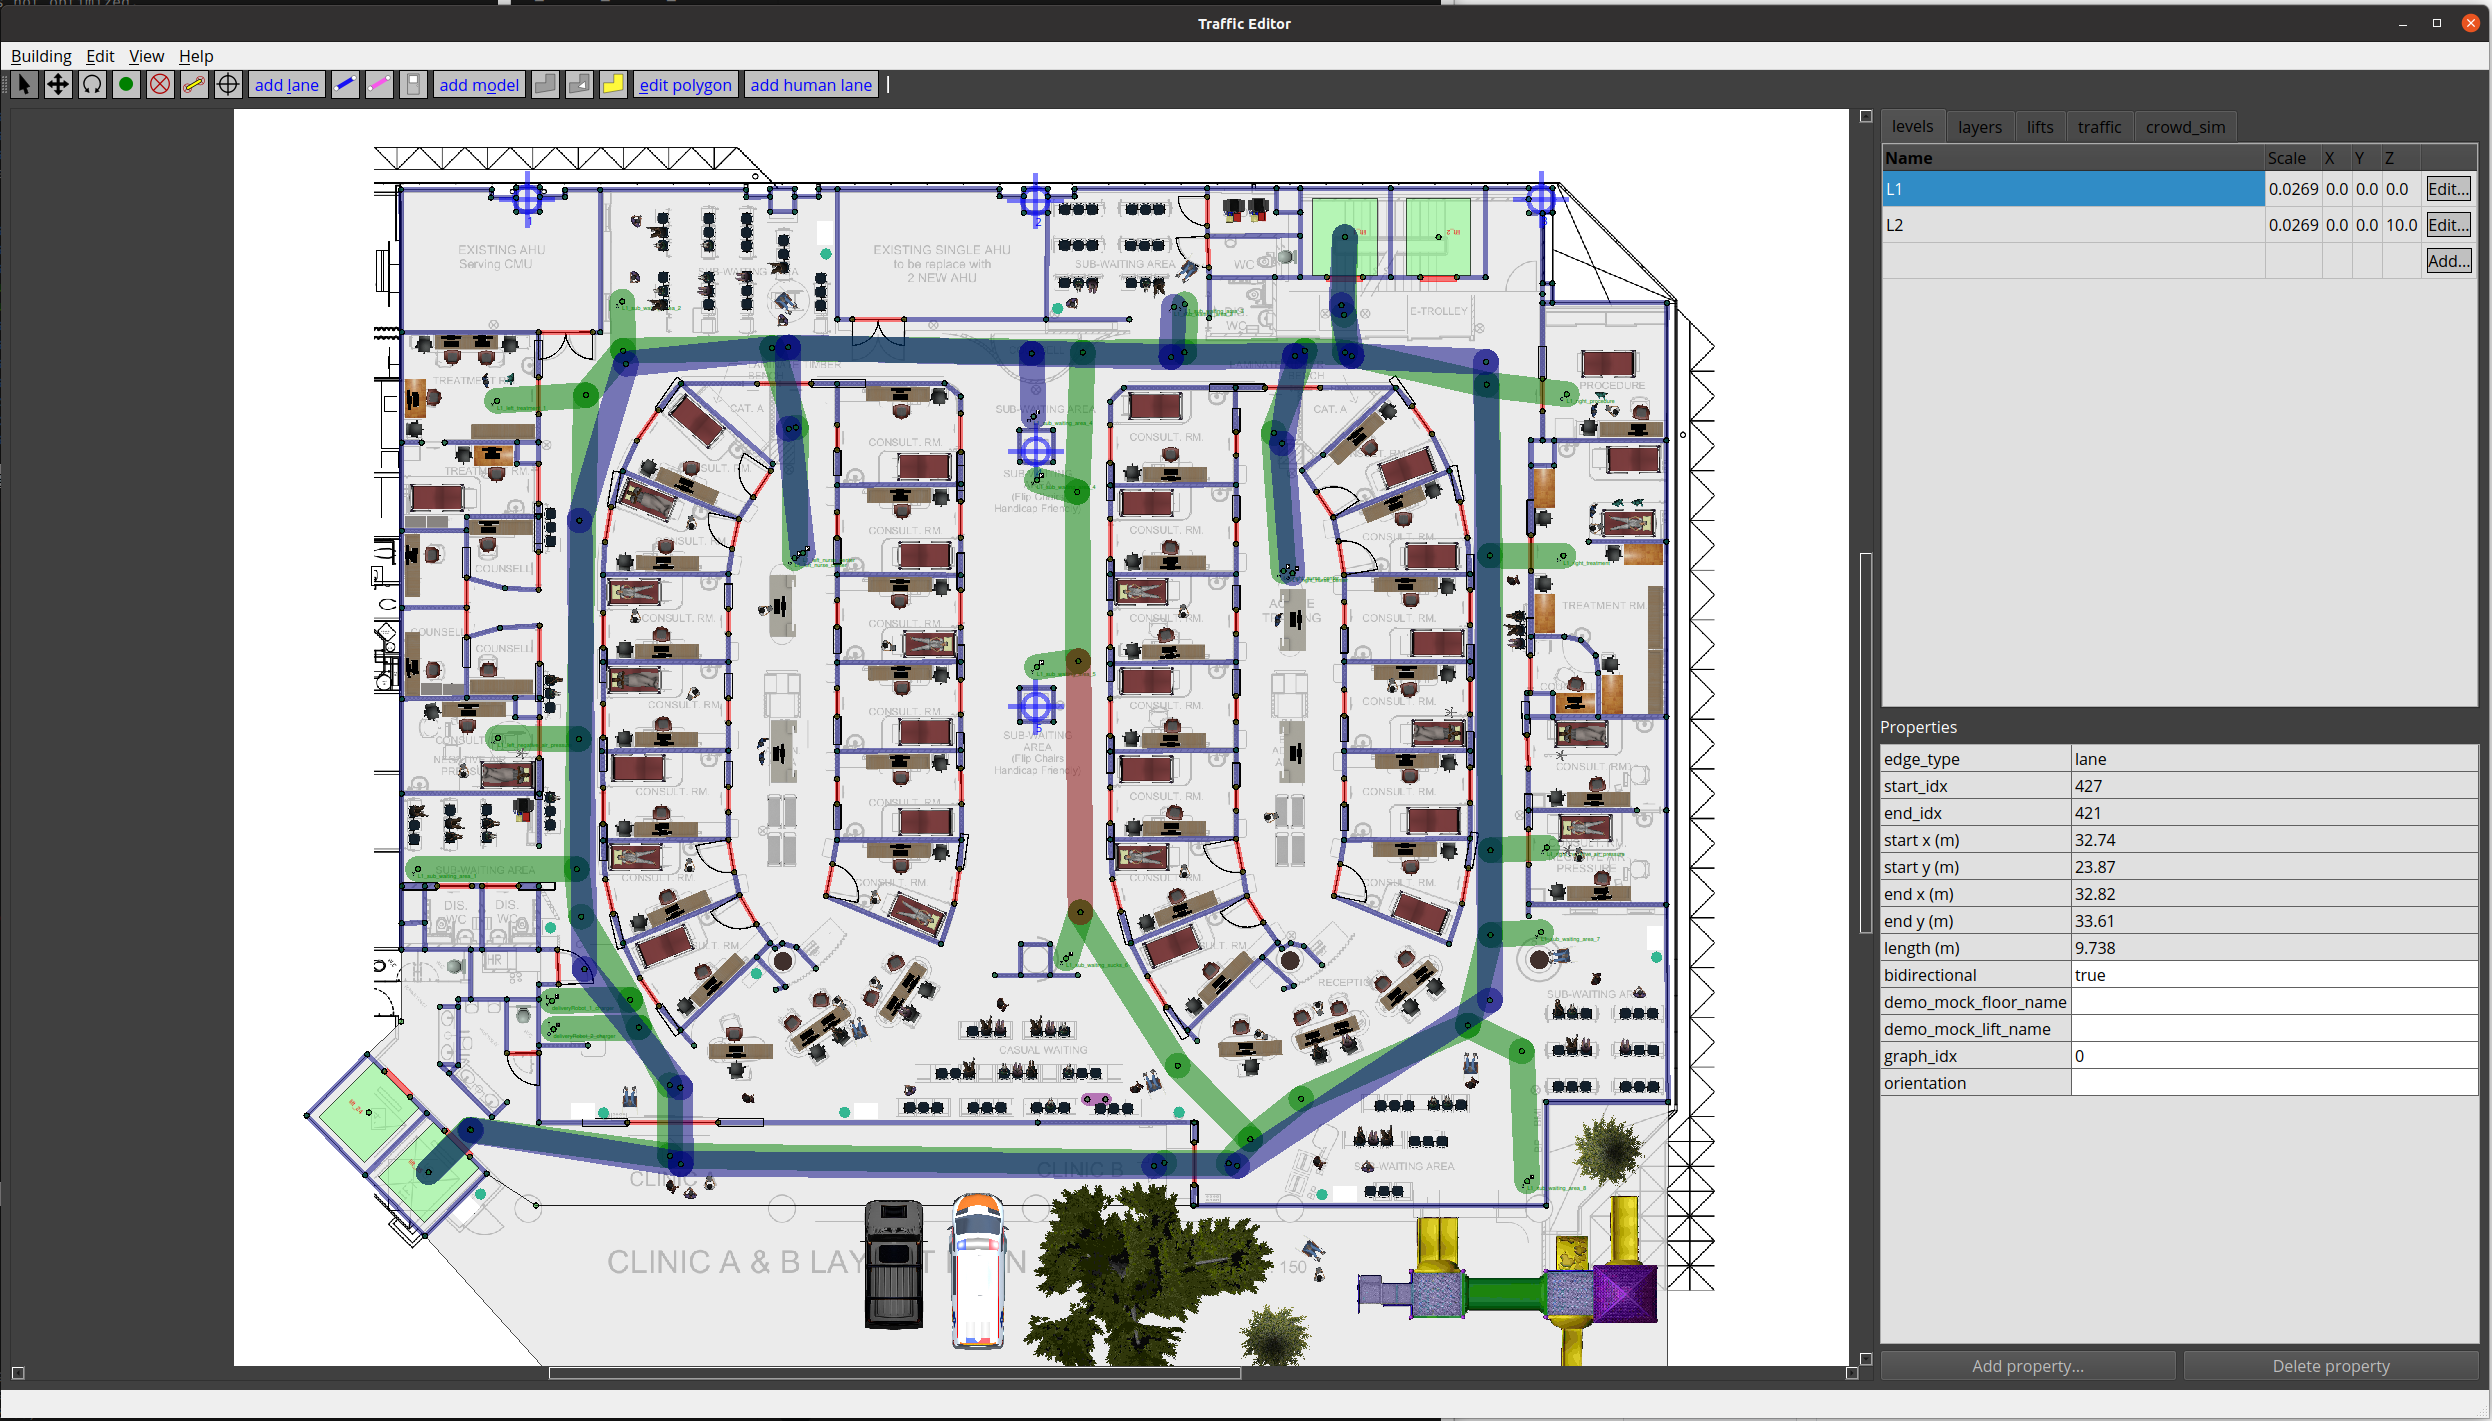
\includegraphics[width=0.8\linewidth]{img/RMF_tut_trafficEditor.png}
		\captionof{figure}{Traffic Editor}
		\label{fig:Traffic Editor}
	\end{figure}\\
	Another version of this software,  \textbf{rmf\_site}\footnote{\href{https://github.com/open-rmf/rmf\_site}{https://github.com/open-rmf/rmf\_site}}, is currently undergoing active deployment.
	\item \textbf{Free Fleet}: An open-source fleet adapter that enables the integration of standalone mobile robots into Open-RMF, allowing the creation of heterogeneous fleets.
	\begin{figure}[h]
		\centering
		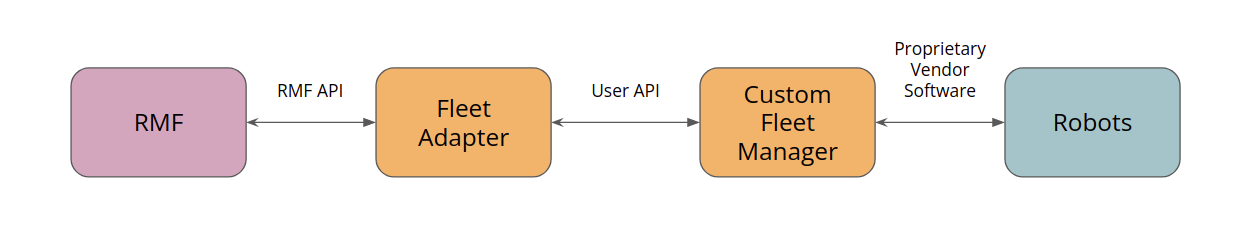
\includegraphics[width=0.8\linewidth]{img/RMF_tut_fleetAdapterTMPL.png}
		\captionof{figure}{Fleet Adapter}
		\label{fig:Fleet Adapter}
	\end{figure}
	\item \textbf{RMF Schedule Visualizer}: An RViz plugin that provides visualization and monitoring of the RMF schedule, enabling users to observe and interact with traffic and task execution in real time.
	\newpage
	\item \textbf{RMF Web UI} : A web-based application for visualization and control of the Robotic Middleware Framework (\texttt{rmf\_core}). It provides a user-friendly interface for monitoring system state and interacting with fleet operations.
	\begin{figure}[h]
		\centering
		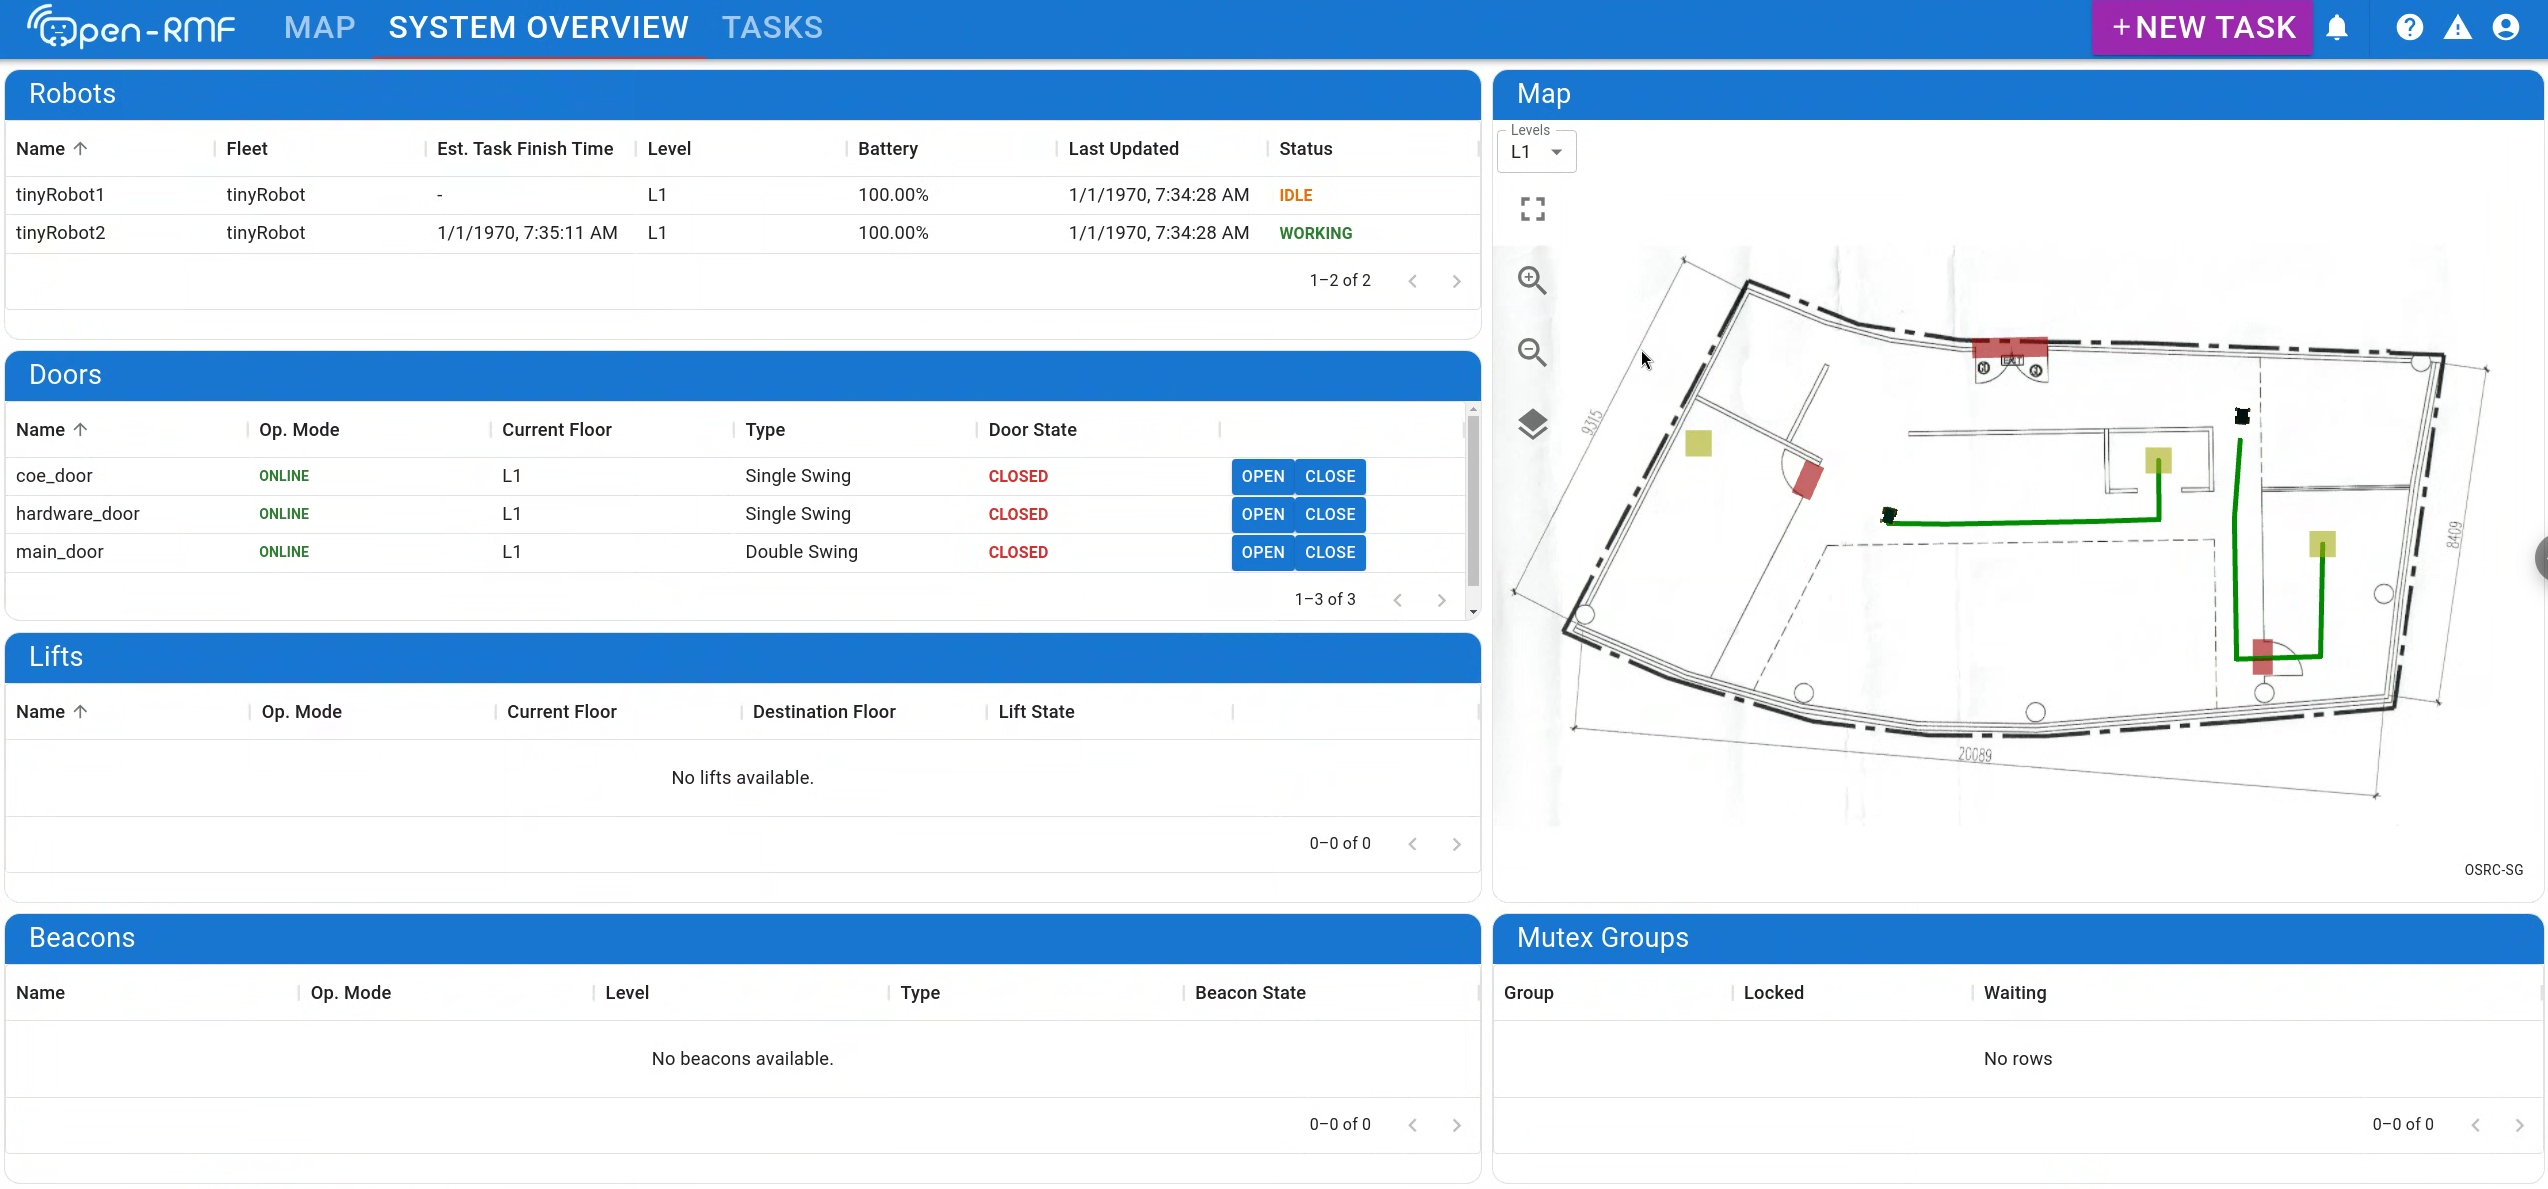
\includegraphics[width=0.8\linewidth]{img/RMF_tut_web.png}
		\captionof{figure}{RMF Web}
		\label{fig:RMF Web}
	\end{figure}
	\item \textbf{RMF Simulation}: A set of Gazebo plugins designed to simulate various aspects of building infrastructure—such as doors, lifts, and crowds—as well as robot behavior, including navigation and interactions with workcells.
	\item \textbf{Simulation assets}: Freely available 3D models and environment assets used to support simulation development and testing in Gazebo.
\end{itemize}

